\documentclass[a4paper,12pt]{article}
\usepackage{amsmath}
\usepackage{amssymb,amsthm,graphicx}
\usepackage{enumitem}
\usepackage{color}
\usepackage{epsfig}
\usepackage{graphics}
\usepackage{pdfpages}
\usepackage{subcaption}
\usepackage[font=small]{caption}
\usepackage[hang,flushmargin]{footmisc} 
\usepackage{float}
\usepackage{booktabs}
\usepackage[mathscr]{euscript}
\usepackage{natbib}
\usepackage{setspace}
\usepackage{mathrsfs}
\usepackage[left=2.7cm,right=2.7cm,bottom=2.7cm,top=2.7cm]{geometry}
%\usepackage{subfig}
\usepackage{graphicx}
\parindent0pt 


% General

\newcommand{\reals}{\mathbb{R}}
\newcommand{\integers}{\mathbb{Z}}
\newcommand{\naturals}{\mathbb{N}}

\newcommand{\pr}{\mathbb{P}}        % probability
\newcommand{\ex}{\mathbb{E}}        % expectation
\newcommand{\var}{\textnormal{Var}} % variance
\newcommand{\cov}{\textnormal{Cov}} % covariance

\newcommand{\law}{\mathcal{L}} % law of X
\newcommand{\normal}{N}        % normal distribution 

\newcommand{\argmax}{\textnormal{argmax}}
\newcommand{\argmin}{\textnormal{argmin}}

\newcommand{\ind}{\mathbbm{1}} % indicator function
\newcommand{\kernel}{K} % kernel function
\newcommand{\wght}{W} % kernel weight
\newcommand{\thres}{\pi} % threshold parameter


% Convergence

\newcommand{\convd}{\stackrel{d}{\longrightarrow}}              % convergence in distribution
\newcommand{\convp}{\stackrel{P}{\longrightarrow}}              % convergence in probability
\newcommand{\convas}{\stackrel{\textrm{a.s.}}{\longrightarrow}} % convergence almost surely
\newcommand{\convw}{\rightsquigarrow}                           % weak convergence


% Theorem-like declarations

\theoremstyle{plain}

\newtheorem{theorem}{Theorem}[section]
\newtheorem{prop}[theorem]{Proposition}
\newtheorem{lemma}[theorem]{Lemma}
\newtheorem{corollary}[theorem]{Corollary}
\newtheorem*{theo}{Theorem}
\newtheorem{propA}{Proposition}[section]
\newtheorem{lemmaA}[propA]{Lemma}
\newtheorem{definition}{Definition}[section]
\newtheorem{remark}{Remark}[section]
\renewcommand{\thelemmaA}{A.\arabic{lemmaA}}
\renewcommand{\thepropA}{A.\arabic{propA}}
\newtheorem*{algo}{Clustering Algorithm}


% Theorem numbering to the left

\makeatletter
\newcommand{\lefteqno}{\let\veqno\@@leqno}
\makeatother


% Heading

\newcommand{\heading}[2]
{  \setcounter{page}{1}
   \begin{center}

   \phantom{Distance to upper boundary}
   \vspace{0.5cm}

   {\LARGE \textbf{#1}}
   \vspace{0.4cm}
 
   {\LARGE \textbf{#2}}
   \end{center}
}


% Authors

\newcommand{\authors}[4]
{  \parindent0pt
   \begin{center}
      \begin{minipage}[c][2cm][c]{5cm}
      \begin{center} 
      {\large #1} 
      \vspace{0.05cm}
      
      #2 
      \end{center}
      \end{minipage}
      \begin{minipage}[c][2cm][c]{5cm}
      \begin{center} 
      {\large #3}
      \vspace{0.05cm}

      #4 
      \end{center}
      \end{minipage}
   \end{center}
}

%\newcommand{\authors}[2]
%{  \parindent0pt
%   \begin{center}
%   {\large #1} 
%   \vspace{0.1cm}
%      
%   #2 
%   \end{center}  
%}


% Version

\newcommand{\version}[1]
{  \begin{center}
   {\large #1}
   \end{center}
   \vspace{3pt}
} 










\begin{document}


\section{Simulations}\label{sec-sim}

\subsection{Size and power simulations}\label{subsec-sim-1}

To assess the finite sample performance of our method, we conduct a number of simulations. In particular, we investigate the test procedure from Section \ref{sec-test-shape}. The simulation design is set up to mimic the situation in the application example of Section \ref{subsec-data-1}: We generate data from the model $Y_t = m(\frac{t}{T}) + \varepsilon_t$ for different time series lengths $T$. The errors $\varepsilon_t$ are drawn from the AR(1) process $\varepsilon_t = a \varepsilon_{t-1} + \eta_t$, where $\eta_t$ are independent and normally distributed with mean $0$ and variance $\sigma_\eta^2$. We set $a = 0.267$ and $\sigma_\eta^2 = 0.35$, thus matching the estimated values obtained in the application of Section \ref{subsec-data-1}. To simulate data under the null $H_0: m^\prime = 0$, we let $m$ be a constant function. In particular, we set $m = 0$ without loss of generality. To generate data under the alternative, we consider the trend functions $m(u) = \beta \, (u - 0.6) \, 1(0.6 \le u \le 1)$ with $\beta = 1.25, 1.875, 2.5$. These functions are broken lines with a kink at $u = 0.6$ and different slopes $\beta$. The slope parameter $\beta$ corresponds to a trend with the value $m(1) = 0.4 \, \beta$ at the right endpoint $u = 1$. We thus consider broken lines with the values $m(1) = 0.5, 0.75, 1.0$. Inspecting the middle panel of Figure \ref{plot-results-app1}, the broken line with the slope $\beta = 2.5$ can be seen to resemble the local linear trend estimates in the real-data example of Section \ref{subsec-data-1} the most (where we neglect the nonlinearities of the local linear fits at the beginning of the observation period). The broken lines with the smaller slopes $\beta = 1.25$ and $\beta = 1.875$ are closer to the null making it harder for our test to detect these alternatives.


To implement our test, we choose $K$ to be an Epanechnikov kernel and define the set $\mathcal{G}_T$ of location-scale points $(u,h)$ as
\begin{align}
\mathcal{G}_T = \big\{ (u, h): & \, \, u = 5k/T \text{ for some } 1 \le k \le T/5 \text{ and } \nonumber \\ & \, \, h = (3+5\ell)/T \text{ for some } 0 \le \ell \le T/20 \big\}. \label{grid-sim-app}
\end{align}
We thus take into account all rescaled time points $u \in [0,1]$ on an equidistant grid with step length $5/T$. For the bandwidth $h = (3 + 5\ell)/T$ and any $u \in [h,1-h]$, the local linear weights $w_{t,T}^\prime(u,h)$ are non-zero for exactly $5 + 10 \ell$ observations. Hence, the bandwidths $h$ in $\mathcal{G}_T$ correspond to effective sample sizes of $5, 15, 25, \ldots$ up to approximately $T/2$ data points. We estimate the long-run error variance $\sigma^2$ by the procedure from Section \ref{subsec-error-var-ar}, setting the tuning parameters $L_1$ and $L_2$ to $\lfloor \sqrt{T} \rfloor$ and $\lfloor 2\sqrt{T} \rfloor$, respectively. To compute the critical values of the test, we simulate $1000$ values of the statistic $\Phi^\prime_T$ defined in Section \ref{subsec-test-shape-test} and compute their empirical $(1-\alpha)$ quantile $q_T^\prime(\alpha)$. 


\begin{table}[t]
\footnotesize{
\begin{center}
\caption{Size of the multiscale test from Section \ref{sec-test-shape} for different sample sizes $T$ and nominal sizes $\alpha$.}
\label{tab:size_shape}
\renewcommand{\arraystretch}{1.2}
% latex table generated in R 3.4.3 by xtable 1.8-2 package
% 
\begin{tabular}{cccc}
  \hline
  & \multicolumn{3}{c}{nominal size $\alpha$} \\
 $T$ & 0.01 & 0.05 & 0.1 \\
 \hline
250 & 0.004 & 0.022 & 0.082 \\ 
  350 & 0.007 & 0.031 & 0.067 \\ 
  500 & 0.011 & 0.056 & 0.086 \\ 
  1000 & 0.011 & 0.060 & 0.098 \\ 
   \hline
\end{tabular}

\end{center}}
\footnotesize{
\begin{center}
\caption{Power of the multiscale test from Section \ref{sec-test-shape} for different sample sizes $T$ and nominal sizes $\alpha$. Each panel corresponds to a different slope parameter $\beta$.}\label{tab:power_shape}
\begin{subtable}[b]{0.32\textwidth}
\centering
\caption{$\beta = 1.25$}\label{tab:power_050_ll_shape}
\renewcommand{\arraystretch}{1.2}
% latex table generated in R 3.4.3 by xtable 1.8-2 package
% 
\begin{tabular}{cccc}
  \hline
  & \multicolumn{3}{c}{nominal size $\alpha$} \\
 $T$ & 0.01 & 0.05 & 0.1 \\
 \hline
250 & 0.107 & 0.223 & 0.358 \\ 
  350 & 0.216 & 0.374 & 0.500 \\ 
  500 & 0.280 & 0.554 & 0.678 \\ 
  1000 & 0.756 & 0.910 & 0.935 \\ 
   \hline
\end{tabular}

\end{subtable}
\begin{subtable}[b]{0.32\textwidth}
\centering
\caption{$\beta = 1.875$}\label{tab:power_075_ll_shape}
\renewcommand{\arraystretch}{1.2}
% latex table generated in R 3.4.3 by xtable 1.8-2 package
% 
\begin{tabular}{cccc}
  \hline
  & \multicolumn{3}{c}{nominal size $\alpha$} \\
 $T$ & 0.01 & 0.05 & 0.1 \\
 \hline
250 & 0.365 & 0.582 & 0.709 \\ 
  350 & 0.644 & 0.779 & 0.845 \\ 
  500 & 0.784 & 0.942 & 0.976 \\ 
  1000 & 0.997 & 1.000 & 1.000 \\ 
   \hline
\end{tabular}

\end{subtable}
\begin{subtable}[b]{0.32\textwidth}
\centering
\caption{$\beta = 2.5$}\label{tab:power_100_ll_shape}
\renewcommand{\arraystretch}{1.2}
% latex table generated in R 3.4.3 by xtable 1.8-2 package
% 
\begin{tabular}{cccc}
  \hline
  & \multicolumn{3}{c}{nominal size $\alpha$} \\
 $T$ & 0.01 & 0.05 & 0.1 \\
 \hline
250 & 0.717 & 0.875 & 0.928 \\ 
  350 & 0.933 & 0.977 & 0.989 \\ 
  500 & 0.989 & 0.999 & 1.000 \\ 
  1000 & 1.000 & 1.000 & 1.000 \\ 
   \hline
\end{tabular}

\end{subtable}
\end{center}}
\vspace{-0.4cm}
\end{table}


Tables \ref{tab:size_shape} and \ref{tab:power_shape} report the simulation results for the sample sizes $T=250,350,500, 1000$ and the significance levels $\alpha = 0.01, 0.05, 0.10$. The sample size $T = 350$ is approximately equal to the time series length $359$ in the real-data example of Section \ref{subsec-data-1}. To produce our simulation results, we generate $S=1000$ samples for each time series length $T$ and carry out the multiscale test for each simulated sample. The entries of Tables \ref{tab:size_shape} and \ref{tab:power_shape} are computed as the number of simulations in which the test rejects divided by the total number of simulations. As can be seen from Table \ref{tab:size_shape}, the actual size of the test is fairly close to the nominal target $\alpha$ even for small values of $T$. Hence, the test has approximately the correct size. Inspecting Table \ref{tab:power_shape}, one can further see that the test has reasonable power properties. For the smallest value $\beta = 1.25$, the deviation from the null is quite small, making it hard for the test to detect the alternative. As a consequence, the power is only moderate for $T=250$ and $T=350$. When we move further away from the null by increasing the slope parameter $\beta$, the power of the test quickly increases. It can also be seen to rapidly get larger as the sample size grows. For the slope $\beta =2.5$ and the sample size $T=350$, which are the values that resemble the real-life data in Section \ref{subsec-data-1} the most, the power of the test is above $92.9\%$ for all significance levels $\alpha$ considered and thus comes quite close to $1$. 

\subsection{Comparison to SiZer}\label{subsec-sim-2}

In this section, we compare the perfomance of the multiscale method and the SiZer for times series as described in \cite{Rondonotti2007}. 

First, we assess the finite sample properties of both methods by computing the size and the power from $1000$ simulated time series.

In order to make comparison between methods more illustrative, we consider the simplest possible scenario: the observations $Y_t, t \in \{1, \ldots, T\}$ are drawn from a model $Y_t = m(\frac{t}{T}) + \varepsilon_t$ where $\{\varepsilon_t\}$ is a stationary and causal AR(1) process
\[ \varepsilon_t = a_1 \varepsilon_{t - 1} + \eta_t
\]
with $|a_1| < 1$. Here $\eta_t$ are i\.i\.d standard normal innovations with zero mean and finite variance $\sigma_\eta^2$. Let $T = 500$ and the true underlying trend function be defined as $m(x) = 2\big(1 - 100(x - 0.5)^2\big)^2$ for $x \in [0.4, 0.6]$ and $m(x) = 0$ for $x \notin [0.4, 0.6]$. Both the SiZer testing procedure of \cite{Rondonotti2007} and our multiscale method are applied to find intervals where $m(\cdot)$ is either increasing or decreasing. The result of the SiZer is the SiZer map, the graphical representation of the multiple testing procedure. Each pixel of this map corresponds to a particular location $u = t/T$ and a particular bandwidth $h$, and the color of this pixel reflects statistical significance of the slope at $(u, h)$ obtained b the following procedure: at each point $(u, h)$, the trend is significantly increasing (or decreasing) if the confidence intervals for the derivative of the underlying function is above (or below) $0$. If the respective confidence interval contains $0$, no statistical inference about this point $(u, h)$ can be made. The exact algorithm for SiZer is provided in the Supplement. 

As the preliminary grid we use the same set $\mathcal{G}_T$ of location-scale points $(u,h)$ as in Section \ref{subsec-sim-2}:
\begin{align}
\mathcal{G}_T = \big\{ (u, h): & \, \, u = 5k/T \text{ for some } 1 \le k \le T/5 \text{ and } \nonumber \\ & \, \, h = (3+5\ell)/T \text{ for some } 0 \le \ell \le T/20 \big\}.
\end{align}
However, we further restrict our attention only to those locations and bandwidths where the number of ``independent blocks'', as cited in \cite{Rondonotti2007}, is not too sparse for reasonable statistical inference. In particular, we calculate $ESS^*$, the Effective Sample Size for correlated data, and consider only the following set:
\begin{align}
\mathcal{G}_T^*  = \big\{ (u, h)\in \mathcal{G}_T| ESS^*(u, h) \geq 5\}\subset \mathcal{G}_T.
\end{align}

Detailed discussion of ``independent blocks'' and $ESS^*$ can be found in \cite{ChaudhuriMarron1999} and \cite{Rondonotti2007}.

The significance level is chosen as $\alpha = 0.05$, and for each simulation the Gaussian quantile for the multiscale method  $q(1 - \alpha)$ is obtained with $1000$ simulated Gaussian versions of the test statistic $\Phi_T$. 

As the kernel function $K$ for both methods  we use the Epanechnikov kernel. Instead of estimating the autocovariances $\gamma(k)$ for SiZer and the long-run error variance $\sigma^2$ for the multiscale test from the data, we use the true theoretical values: $\widehat{\gamma}(k) = \gamma(k) = \frac{\sigma_\eta^2}{1 - a_1^2}a_1^{|k|}$ and $\widehat{\sigma}^2 = \sigma^2 = \frac{\sigma_\eta^2}{(1 - a_1)^2}$.

To produce our simulation results, we generate $S=1000$ samples for each time series length $T$ and carry out the multiscale test and SiZer test for each simulated sample. As in Section \ref{subsec-sim-1}, for the multiscale test the entries of Tables \ref{tab:size_comparison} and \ref{tab:power_comparison} are computed as the number of simulations in which the test rejects divided by the total number of simulations. For the SiZer, the entries are calculated as the number of simulations in which it detects at least one pair location-bandwidth $(u,h)$ with statistically significant increase or decrease divided by the total number of simulations.

As in Section \ref{subsec-sim-1}, we can see from Table \ref{tab:size_comparison}, the multiscale test has approximately correct size while SiZer finds statistical significance under the null in roughly $20\%$ of the cases. This observation suggests that SiZer is more liberal, identifying all potential points of increase and decrease for further analysis, whereas our test is more persistent and stable.

As can be expected, the significant advantage of the multiscale method in terms of size come at a cost in terms of power. However, the loss in power is not very pronounced for sufficiently big sample sizes $T$. Examining Table \ref{tab:power_comparison}, we can see that...


As noted in \cite{HannigMarron2006}, the classic definition of the size of the test that was discussed above may not be applicable for the purpose of assessing finite sample properties of SiZer. In particular, some of the SiZer maps may have a small number of pixels where the method suggests the slope is statistically significant, when, in fact, the underlying trend function is flat.

From Figure \ref{fig:comparison_SiZer} we can infer that see that our multiscale procedure works much better in the case of negative coefficient $a_1$ and has relatively same efficiency for positive coefficients $a_1$.

\begin{figure}
\begin{subfigure}{.5\textwidth}
  \centering
  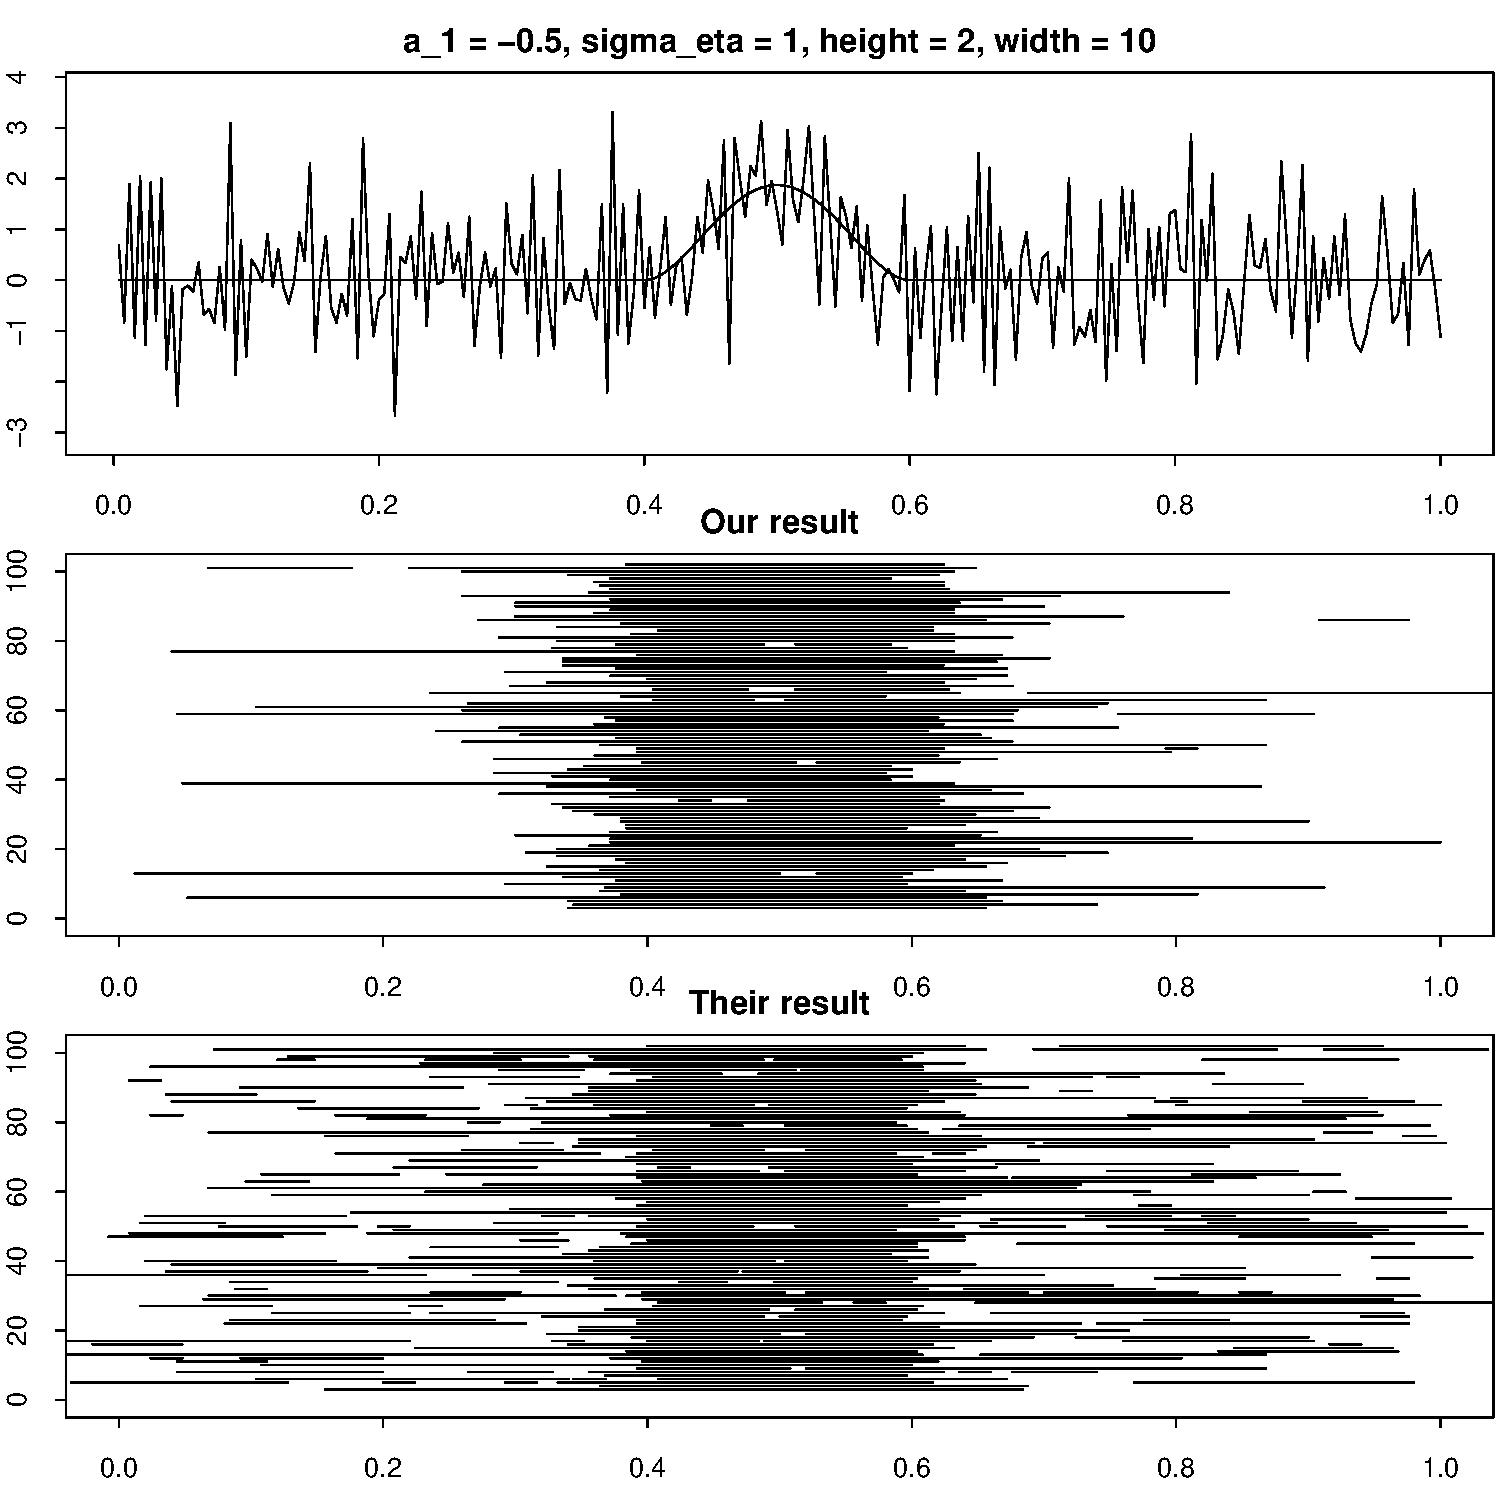
\includegraphics[width=.9\linewidth]{Plots/min_int_with_T_250_a1_-05_height_2_width_10.pdf}
  \caption{$a_1 = -0.5$}
  \label{fig:sfig1}
\end{subfigure}%
\begin{subfigure}{.5\textwidth}
  \centering
  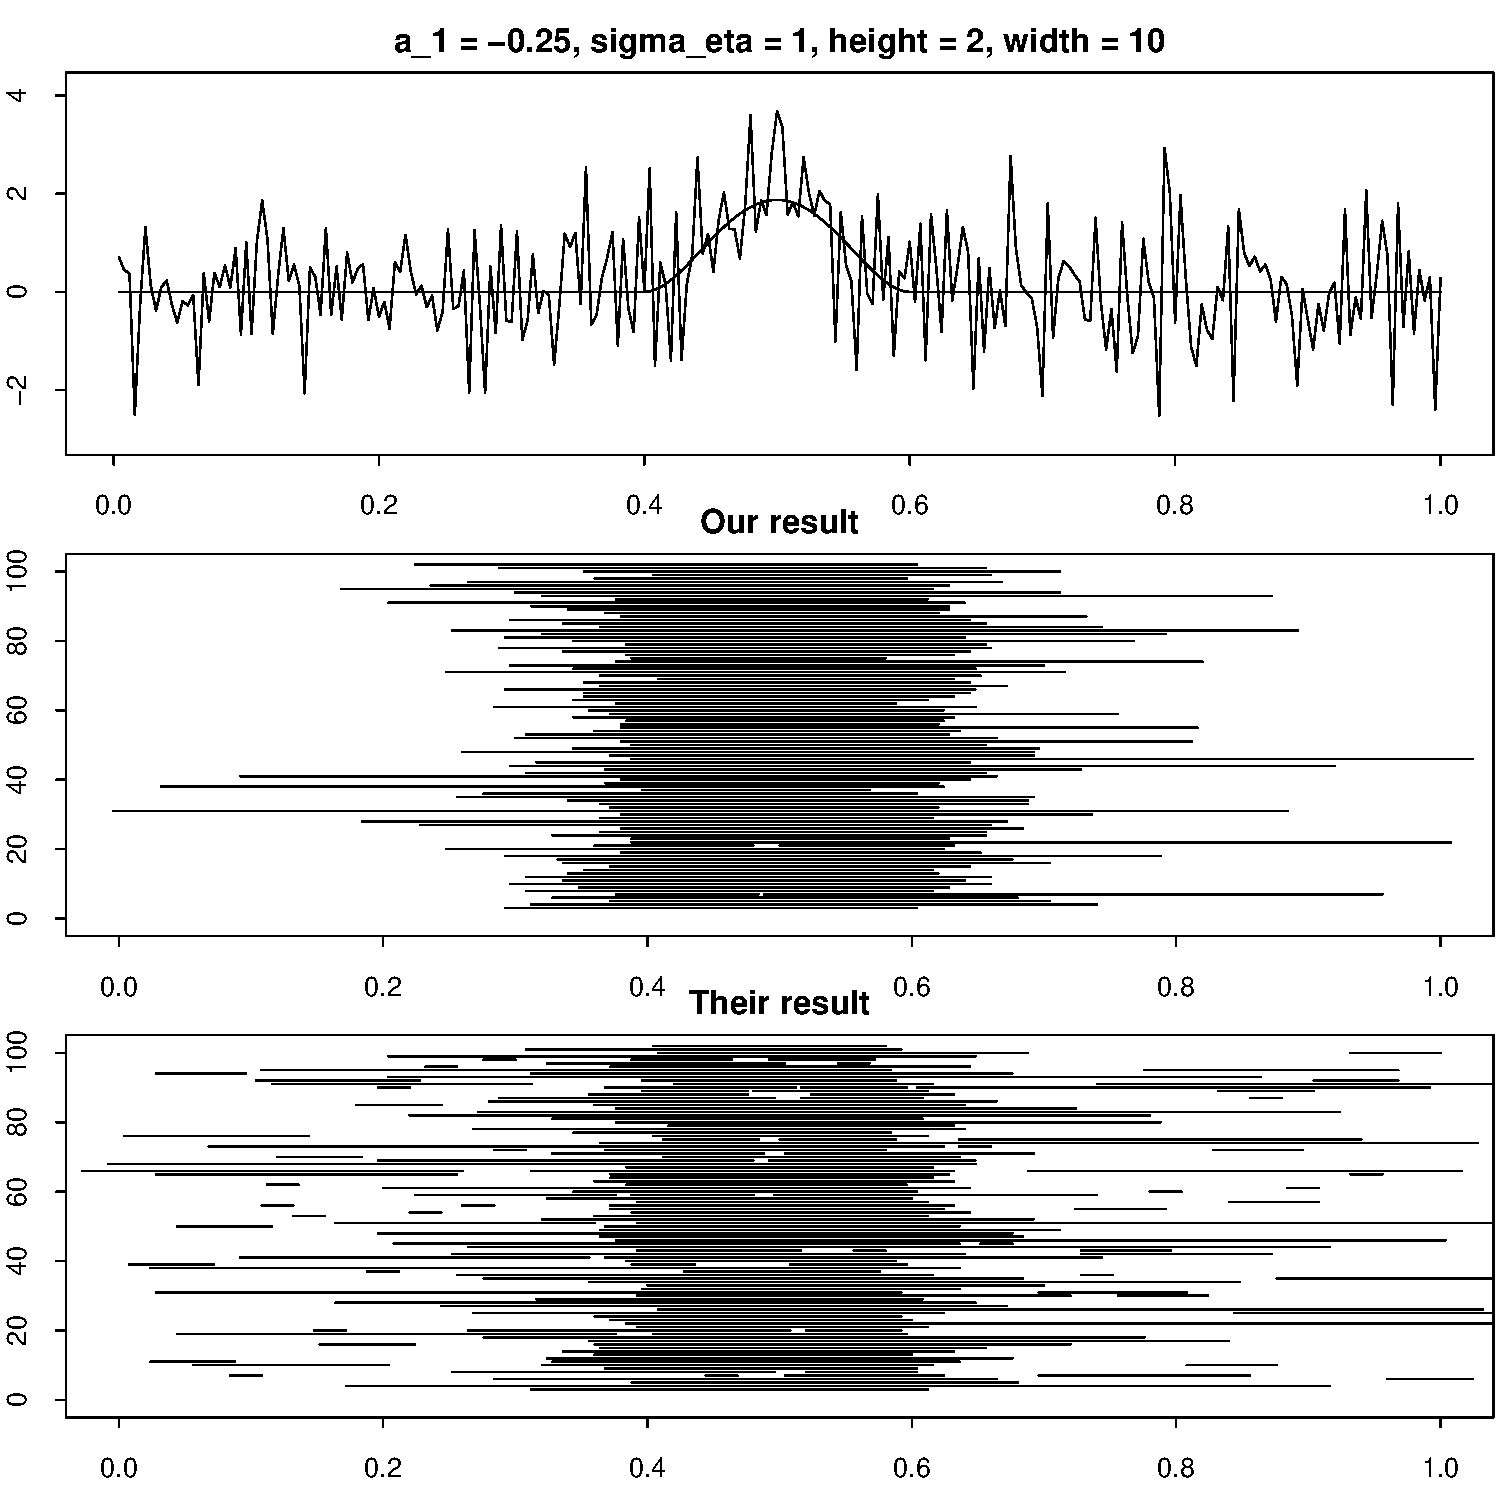
\includegraphics[width=.9\linewidth]{Plots/min_int_with_T_250_a1_-025_height_2_width_10.pdf}
  \caption{$a_1 = -0.25$}
  \label{fig:sfig2}
\end{subfigure}\\
\begin{subfigure}{.5\textwidth}
  \centering
  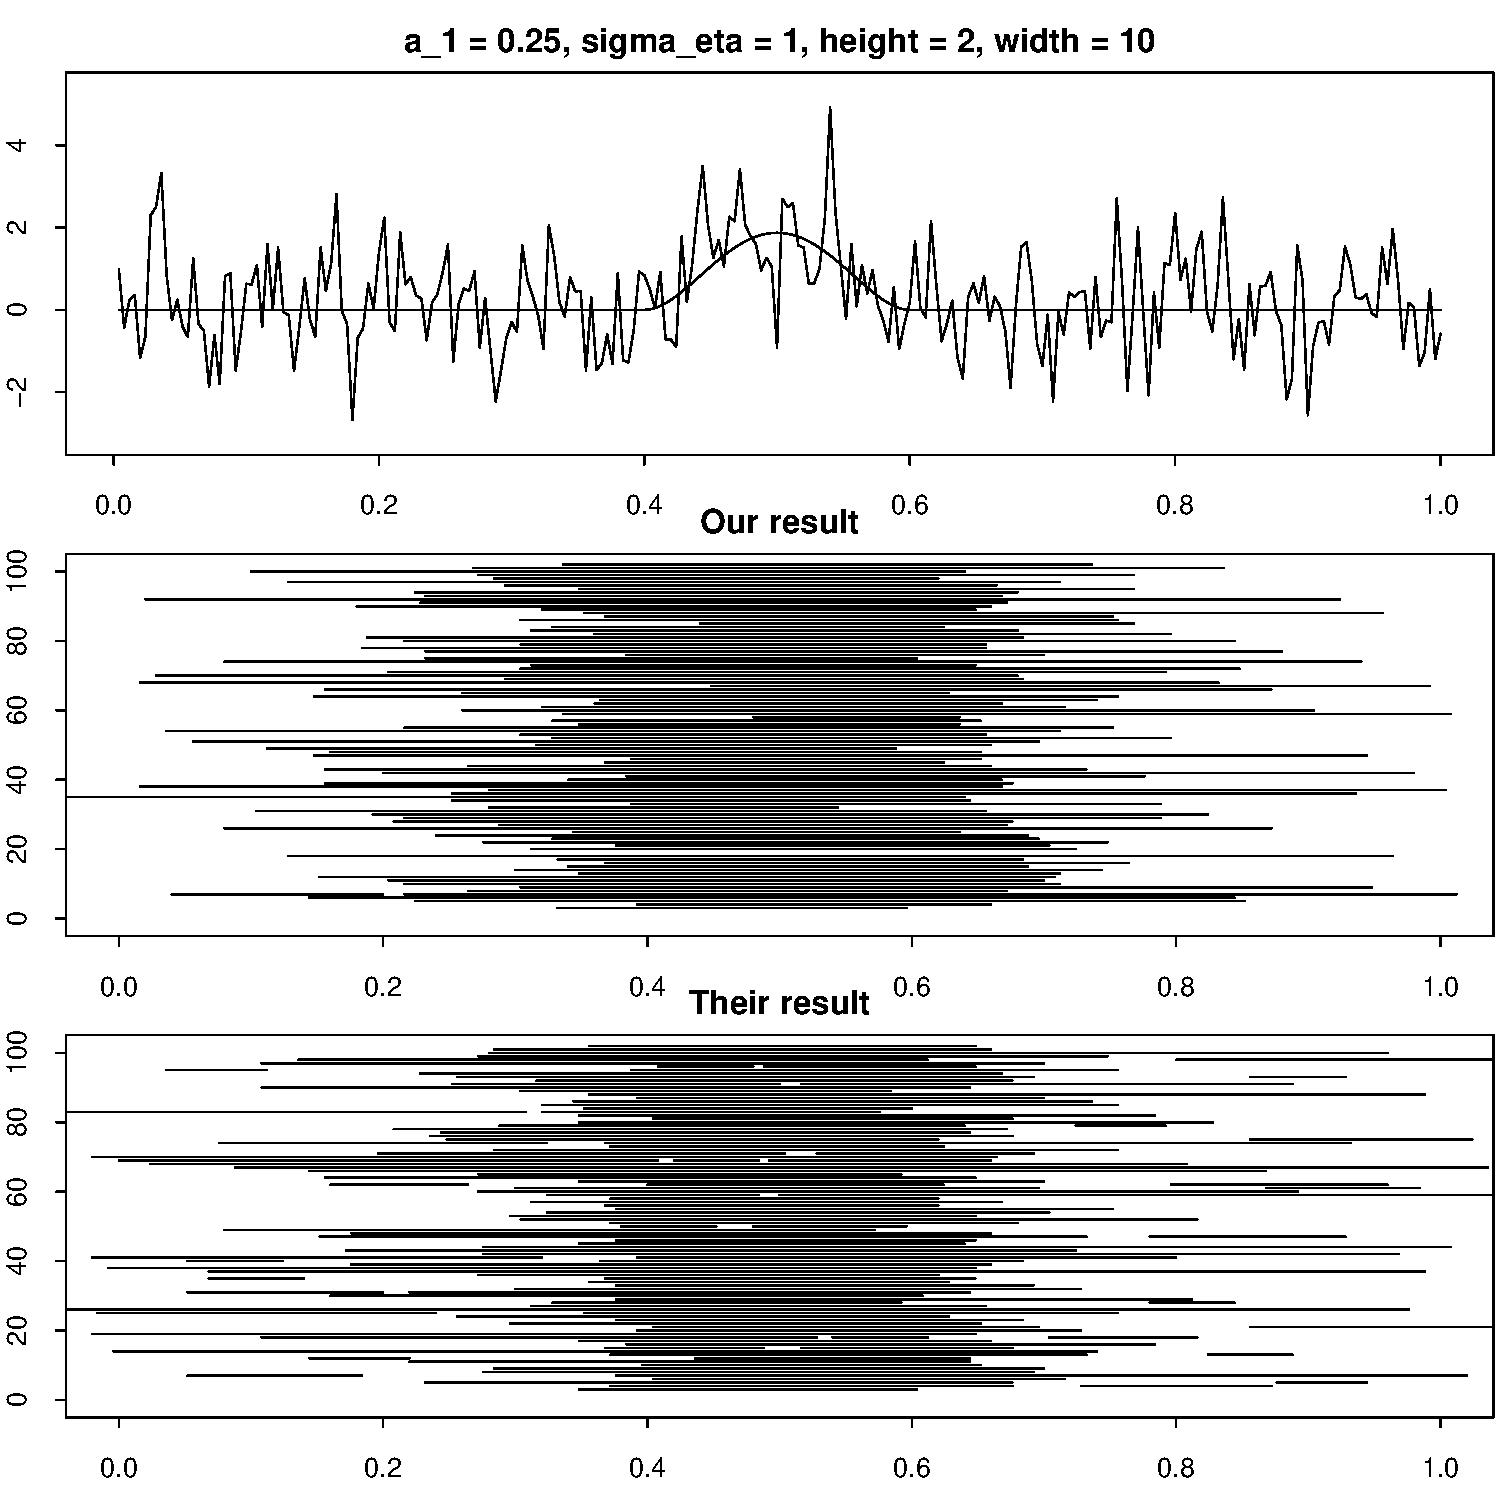
\includegraphics[width=.9\linewidth]{Plots/min_int_with_T_250_a1_025_height_2_width_10.pdf}
  \caption{$a_1 = 0.25$}
  \label{fig:sfig3}
\end{subfigure}%
\begin{subfigure}{.5\textwidth}
  \centering
  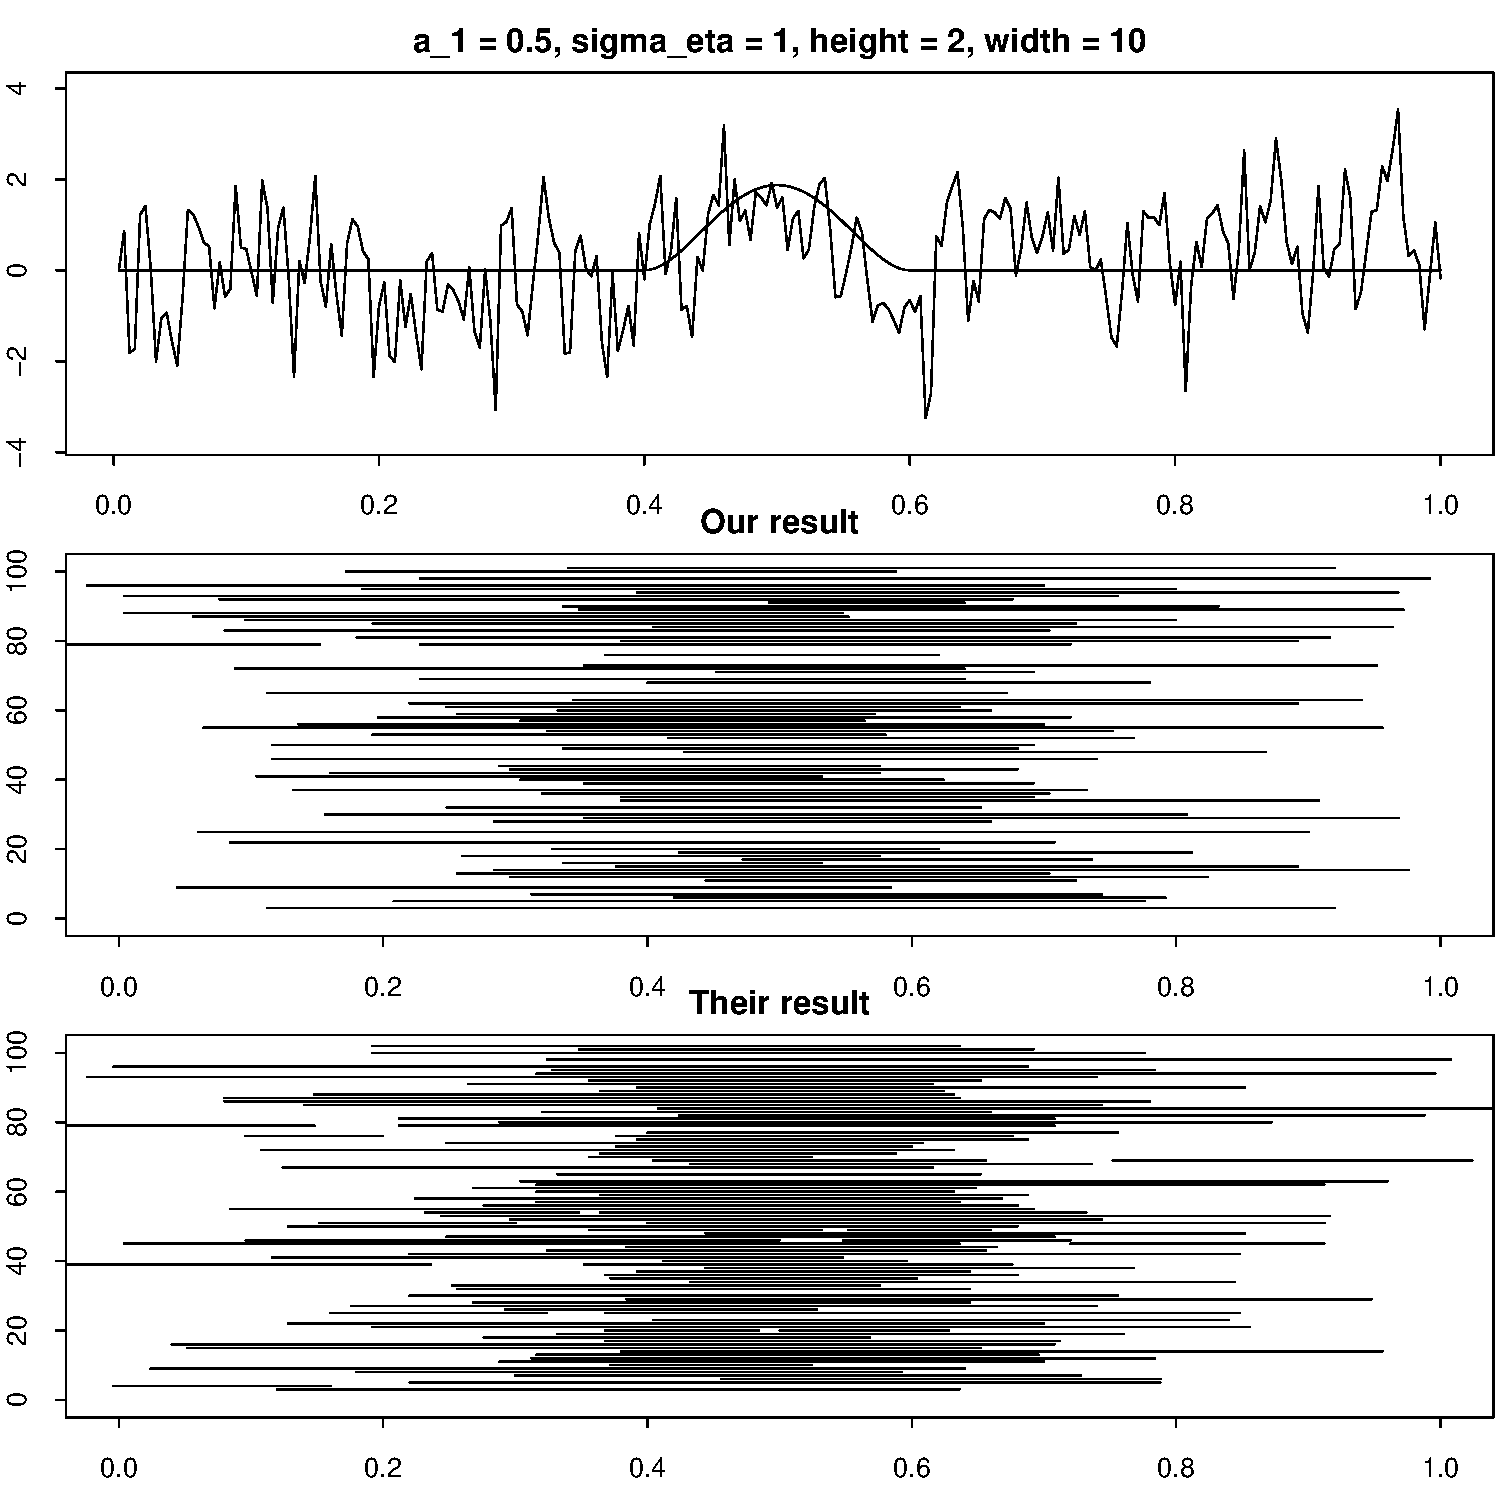
\includegraphics[width=.9\linewidth]{Plots/min_int_with_T_250_a1_05_height_2_width_10.pdf}
  \caption{$a_1 = 0.5$}
  \label{fig:sfig4}
\end{subfigure}\\
\caption{Summary of the simulation results for Section \ref{subsec-sim-2} for different model settings. In these settings the underlying trend function is $m(x) = 2\big(1 - 100(x - 0.5)^2\big)^2$ for $x \in [0.4, 0.6]$ and $m(x) = 0$ for $x \notin [0.4, 0.6]$. The errors are generated from an AR(1) process with coefficients $a_1 \in \{-0.5, -0.25, 0.25, 0.5\}$. Each of the figures correspond to one of the coefficients $a_1$ which are provided below the figures. The upper panel on each figure shows an example of the time series generated by the model. The middle panel depicts the union of the minimal intervals in the set $\Pi_T$ produced by the multiscale test for each of the 100 runs. The lower panel presents the regions where SiZer detected increase or decrease of the underlying trend function for each of the 100 runs.}
\label{fig:comparison_SiZer}
\end{figure}

\section{Applications}\label{sec-data}


In what follows, we illustrate the multiscale methods from Sections \ref{sec-test-shape} and \ref{sec-test-equality} by two real-data examples. In the first example, we apply the test method from Section \ref{sec-test-shape} to a long time series of temperature data from Central England. In the second, we analyse a sample of temperature time series from 34 different weather stations in Great Britain with the help of the methods from Section \ref{sec-test-equality}. 


\subsection{Analysis of Central England temperature data}\label{subsec-data-1} 


\begin{figure}[t]
\centering
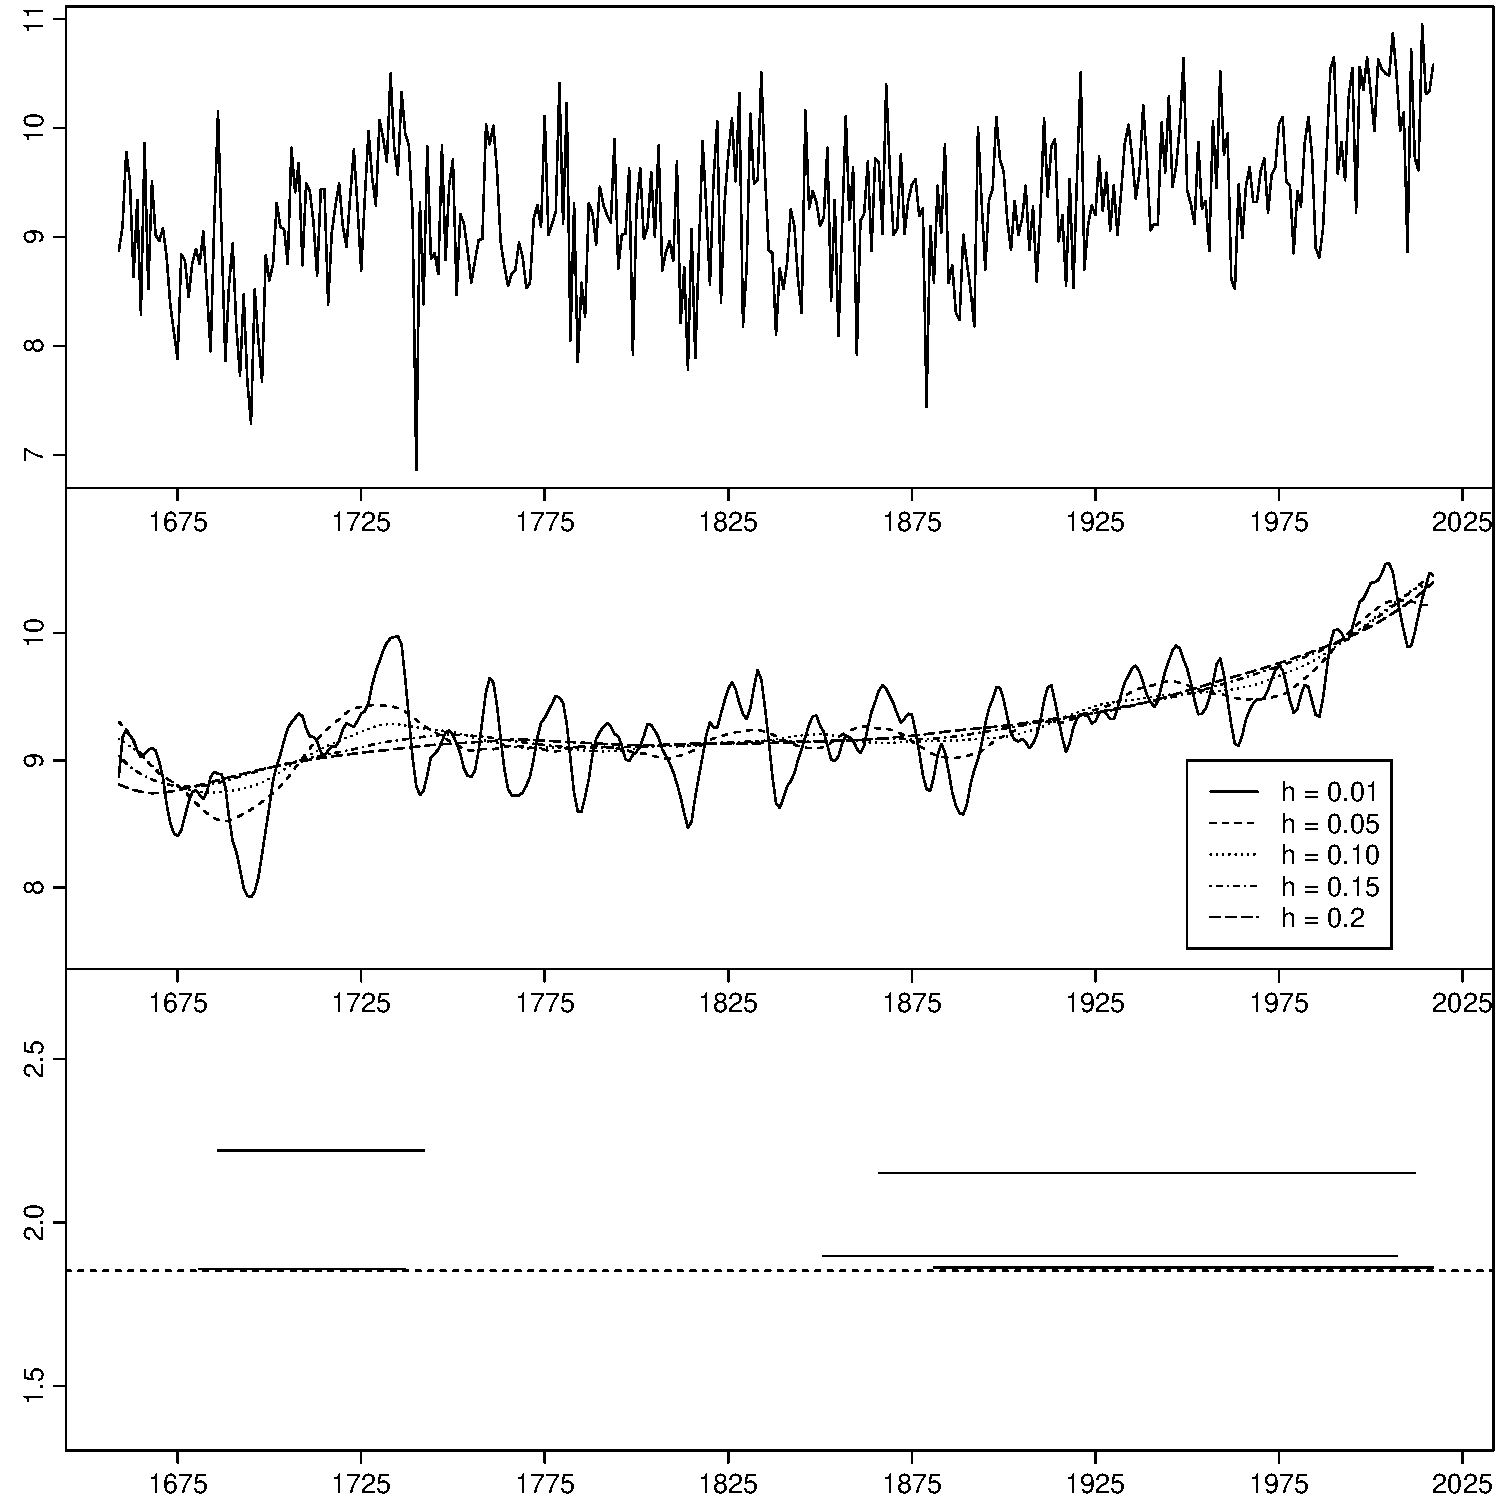
\includegraphics[width=0.8\textwidth]{Plots/threegraphics_testing_constant_method_ll.pdf}
\caption{Summary of the application results for Section \ref{subsec-data-1}. The upper panel shows the Central England mean temperature time series. The middle panel depicts local linear kernel estimates of the time trend for a number of different bandwidths $h$. The lower panel presents the minimal intervals in the set $\Pi_T^+$ produced by the multiscale test. These are $[1681,1737]$, $[1686,1742]$, $[1851,2007]$, $[1866,2012]$ and $[1881,2017]$.}\label{plot-results-app1}
\end{figure}


\enlargethispage{0.2cm}
The analysis of time trends in long temperature records is an important task in climatology. Information on the shape of the trend is needed in order to better understand long-term climate variability. The Central England temperature record is the longest instrumental temperature time series in the world. It is a valuable asset for analysing climate variability over the last few hundred years. The data is publicly available on the webpage of the UK Met Office. A detailed description of the data can be found in \cite{Parker1992}. For our analysis, we use the dataset of yearly mean temperatures which consists of $T=359$ observations covering the years from $1659$ to $2017$. We assume that the data follow the nonparametric trend model 
\[ Y_t = m\Big(\frac{t}{T}\Big) + \varepsilon_t, \]
where $m$ is the unknown time trend of interest. The error process $\{ \varepsilon_t \}$ is supposed to have the AR(1) structure $\varepsilon_t = a \varepsilon_{t-1} + \eta_t$, where $\eta_t$ are i.i.d.\ innovations with mean $0$ and variance $\sigma_\eta^2$. As pointed out in \cite{Mudelsee2010} among others, this is the most widely used error model for discrete climate time series. We estimate the parameters $a$ and $\sigma_\eta^2$ as described in Section \ref{subsec-error-var-ar} which yields the estimates $\widehat{a} \approx 0.267$ and $\widehat{\sigma}_\eta^2 \approx 0.35$.


With the help of our multiscale method from Section \ref{sec-test-shape}, we test the null hypothesis $H_0: m^\prime = 0$, that is, the hypothesis that $m$ is constant. To do so, we set the significance level to $\alpha = 0.05$ and implement the test in exactly the same way as in the simulations of Section \ref{sec-sim}. The results are presented in Figure \ref{plot-results-app1}. The upper panel shows the raw temperature time series, whereas the middle panel depicts local linear kernel estimates of the trend $m$ for different bandwidths $h$. As one can see, the shape of the estimated time trend strongly differs with the chosen bandwidth. When the bandwidth is small, there are many local increases and decreases in the estimated trend. When the bandwidth is large, most of these local variations get smoothed out. Hence, by themselves, the nonparametric fits do not give much information on whether the trend $m$ is increasing or decreasing in certain time regions. 


Our multiscale test provides this kind of information, which is summarized in the lower panel of Figure \ref{plot-results-app1}. The plot depicts the minimal intervals contained in the set $\Pi_T^+$ which is defined in Section \ref{subsec-test-shape-theo}. The set of intervals $\Pi_T^-$ is empty in the present case. The height at which a minimal interval $I_{u,h} = [u-h,u+h] \in \Pi_t^+$ is plotted indicates the value of the corresponding (additively corrected) test statistic $\widehat{\psi}^\prime_T(u,h) / \widehat{\sigma} - \lambda(h)$. The dashed line specifies the critical value $q_T^\prime(\alpha)$, where $\alpha = 0.05$ as already mentioned above. According to Proposition \ref{prop-test-shape-2}, we can make the following simultaneous confidence statement about the collection of minimal intervals in $\Pi_T^+$. We can claim, with confidence of about $95\%$, that the trend function $m$ has some increase on each minimal interval. More specifically, we can claim with this confidence that there has been some upward movement in the trend both in the period from around $1680$ to $1740$ and in the period from about $1880$ onwards. Hence, our test in particular provides evidence that there has been some warming trend in the period over approximately the last $140$ years. On the other hand, as the set $\Pi_T^-$ is empty, there is no evidence of any downward movement of the trend.  

\bibliographystyle{ims}
{\small
\setlength{\bibsep}{0.55em}
\bibliography{bibliography}}
\end{document}
